\documentclass[tikz,border=2pt]{standalone}
\usepackage{amsmath,amssymb}
\usepackage{tikz}
\usetikzlibrary{arrows.meta}

\begin{document}
% The hierarchy of algebraic structures: each step down adds an axiom (or a second operation).
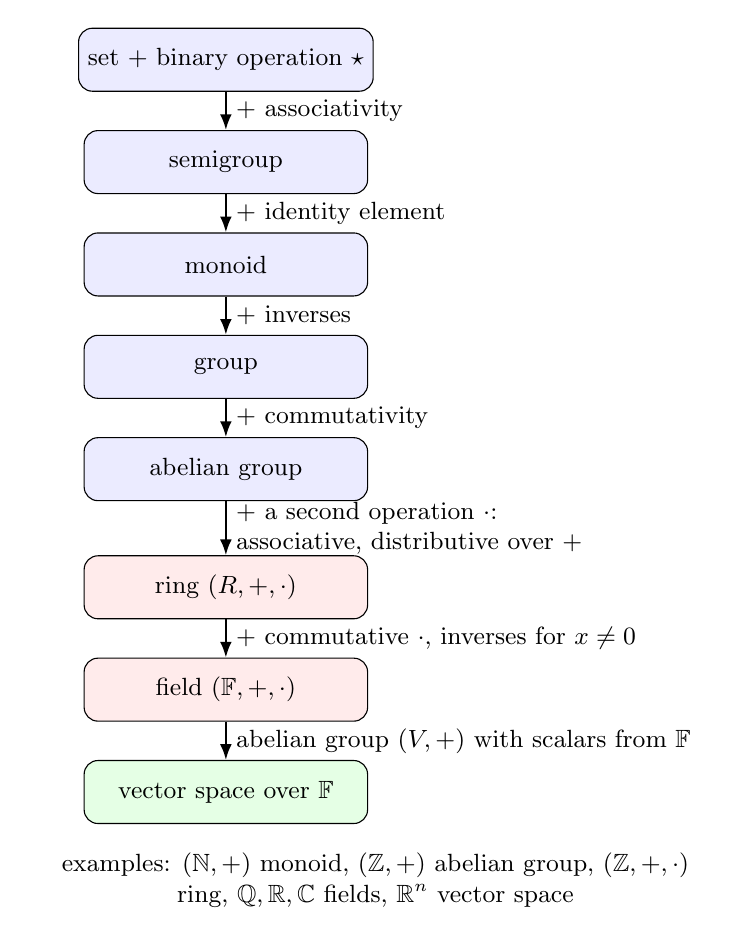
\begin{tikzpicture}[every node/.style={font=\small}, >={Latex[length=2mm]}, box/.style={draw, rounded corners=5pt, minimum width=3.6cm, minimum height=0.8cm, fill=blue!8}, lab/.style={midway, right, font=\small, align=left}]
	\node[box] (set) at (0,0) {set $+$ binary operation $\star$};
	\node[box] (sg) at (0,-1.3) {semigroup};
	\node[box] (mo) at (0,-2.6) {monoid};
	\node[box] (gr) at (0,-3.9) {group};
	\node[box] (ab) at (0,-5.2) {abelian group};
	\node[box, fill=red!8] (ri) at (0,-6.7) {ring $(R,+,\cdot)$};
	\node[box, fill=red!8] (fi) at (0,-8.0) {field $(\mathbb{F},+,\cdot)$};
	\node[box, fill=green!10] (vs) at (0,-9.3) {vector space over $\mathbb{F}$};
	\draw[->, thick] (set) -- (sg) node[lab] {$+$ associativity};
	\draw[->, thick] (sg) -- (mo) node[lab] {$+$ identity element};
	\draw[->, thick] (mo) -- (gr) node[lab] {$+$ inverses};
	\draw[->, thick] (gr) -- (ab) node[lab] {$+$ commutativity};
	\draw[->, thick] (ab) -- (ri) node[lab] {$+$ a second operation $\cdot$:\\ associative, distributive over $+$};
	\draw[->, thick] (ri) -- (fi) node[lab] {$+$ commutative $\cdot$, inverses for $x\neq0$};
	\draw[->, thick] (fi) -- (vs) node[lab] {abelian group $(V,+)$ with scalars from $\mathbb{F}$};
	\node[anchor=north, align=flush center, text width=8.6cm] at (1.9,-9.95) {examples: $(\mathbb{N},+)$ monoid, $(\mathbb{Z},+)$ abelian group, $(\mathbb{Z},+,\cdot)$ ring, $\mathbb{Q},\mathbb{R},\mathbb{C}$ fields, $\mathbb{R}^n$ vector space};
\end{tikzpicture}
\end{document}
